% ------------------------------------------------------------------------------
\section{Desenvolvimento} \label{des}
    
    O PTP provê um método padrão para sincronizar dispositivos em uma rede com precisão de sub-micro segundo. Ele provê não apenas compatibilidade entre sistemas heterogêneos, mas também alta precisão em relação a sincronização dos tempos de relógio. O processo de sincronização é contínuo, pois diversos fatores podem levar dois relógios idênticos a apresentarem valores diferentes e consequentemente perderem sincronia, causas como diferenças na temperatura e frequência podem afetar a qualidade da sincronização.
	
	PTP provê uma sincronização tolerante à falha para diferentes relógios na mesma rede. Algumas vantagens deste protocolo são: pouco consumo de banda e pouco consumo de processamento \cite{Committee2008}. Isto é conseguido através do uso do PTP. O PTP é um protocolo baseado na troca de mensagens que pode ser implementado em redes de comutação de pacotes, incluindo, mas não limitado as redes {\it Ethernet}.
	
	Sua operação inicia-se com o envio de um pacote de sincronização, que é enviado do mestre aos escravos de tempos em tempos, caso seja optado por uma sincronização em um passo, então o {\it timestamp} é registrado e enviado na própria mensagem de sincronização, porém a sincronização também pode ser feita em dois passos. Utilizando dois passos, um pacote {\it Follow Up} também deve ser enviado pelo mestre. Este pacote conterá um {\it timestamp},  que possui o tempo exato em que a mensagem de sincronização deixou o mestre, propiciando assim uma maior precisão, já que o {\it timestamp} poderá ser registrado em camadas mais próximas ao meio físico, o que sofre menos interferências não determinísticas e permite uma maior precisão. A figura 2 mostra as mensagens que são trocadas entre os dispositivos da rede.
	
	
		\begin{figure}[ht]
		\begin{center}
		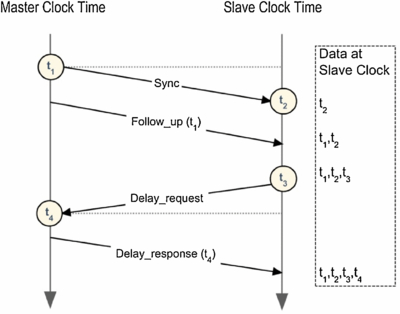
\includegraphics[scale=0.6,width=7cm]{fig/ptp_schema.png}
		\caption{Troca de mensagens efetuadas segundo o protocolo PTP \cite{DelRio2012}}
		\end{center}
		\end{figure}
		
	Após uma visão geral do funcionamento do protocolo, exploraremos melhor seus passos para realizar a sincronização entre os nodos da rede. Os passos seguem a seguinte ordem:
		
		
	\begin{enumerate}
	\item O nodo mestre envia uma mensagem de sincronização ao nodo escravo e registra o tempo de envio  $t{_1}$.
	\item O escravo recebe a mensagem de sincronização e registra o tempo de recebimento da mesma $t{_2}$.
	\item O nodo mestre transporta ao nodo escravo o tempo $t{_1}$ registrado através da seguinte forma:
	\begin{itemize}
	\item Inserindo o {\it timestamp} $t{_1}$ na mensagem de sincronização (um-passo). Este método requer algum processo de hardware para melhor precisão.
	\item Inserindo o {\it timestamp} $t{_1}$ em uma mensagem de {\it Follow Up} (dois-passos).
	\end{itemize}
	\item O nodo escravo envia uma mensagem de requisição de atraso para o nodo mestre e registra o tempo de envio $t{_3}$.
	\item O nodo mestre recebe a mensagem de requisição de atraso e registra
	\item O nodo mestre transmite ao nodo escravo o {\it timestamp} $t{_4}$ inserindo-o em uma mensagem de resposta de atraso.
	\end{enumerate}
		
		Após realizar estas trocas de mensagens o nodo escravo possuirá quatro {\it timestamps} e a partir dos mesmos será possível obter o {\it offset} entre o tempo registrado no nodo mestre em comparação com o tempo registrado no nodo escravo, e assim o atraso da rede, tempo necessário para pacotes trafegarem por pelo link entre dois nodos comunicantes.
		
		O atraso no link pode ser calculado da seguinte maneira : 
		

		\begin{equation}
			{\beta} =  t{_2} - t{_1}
		\end{equation}
		
		\begin{equation}
			{\gamma} =  t{_4} - t{_3}
		\end{equation}
							
		%Mestre-Escravo = tms = t2 -t1
		%Escravo-Mestre = tsm = t4 - t3
		
		O $\beta$ representa o atraso no sentido Mestre-Escravo, enquanto que o $\gamma$ representa o atraso no sentido Escravo-Mestre. Em cada caso, a diferença nos tempos se refere aos tempos tomados por dois relógios diferentes. No entanto, caso se assuma, que o atraso em uma direção é o mesmo atraso que no sentido oposto, então as duas equações podem ser combinadas na seguinte equação.
		

		\begin{equation}
			{\alpha} =  \frac{( \beta ) + ( \gamma )}{2}
		\end{equation}
						
		%Delay = (( t2 - t1 ) + ( t4 - t3 ) )* 0,5
		
		
		Assim sendo, temos representado por $\alpha$ o atraso da rede, e podemos obter o {\it offset} do relógio do nodo escravo através da seguinte equação:
		

		\begin{equation}
			{\phi} =  t{_2} - ( t{_1} + {\alpha} )
		\end{equation}
				
		%Offset = t2 - ( t1 + Delay )
		
		
		Ou realizando substituições e otimizações, sendo $\phi$ equivalente ao {\it offset} a partir do mestre:
		
		\begin{equation}
			{\phi} = \frac{( \beta ) - ( \gamma )}{2} 
		\end{equation}
		
		Caso dois conjuntos de mensagens de sincronização e de {\it Follow Up} sejam enviadas, então o {\it drift} entre os dois relógios pode ser descoberto através da comparação da variação de tempo entre duas mensagens de sincronização sucessivas, como prossegue.
		
		\begin{equation}
			{\rho} = \frac{( t_{escravo} ) - ( t_{mestre} )}{t_{mestre}} 
		\end{equation}	
	
		$\rho$ representa o {\it drift}, ou escorregamento, entre os relógios mestre e escravo, sendo os tempos equivalentes aos tempos marcados nos mesmos.
		
		Dado este aspecto teórico, chegou-se a máquina de estados apresentada na Figura 3. Esta foi utilizada na implementação do protocolo PTP utilizando o Sistema Operacional EPOS \cite{Guto}.
		\begin{figure*}[ht]
		\begin{center}
		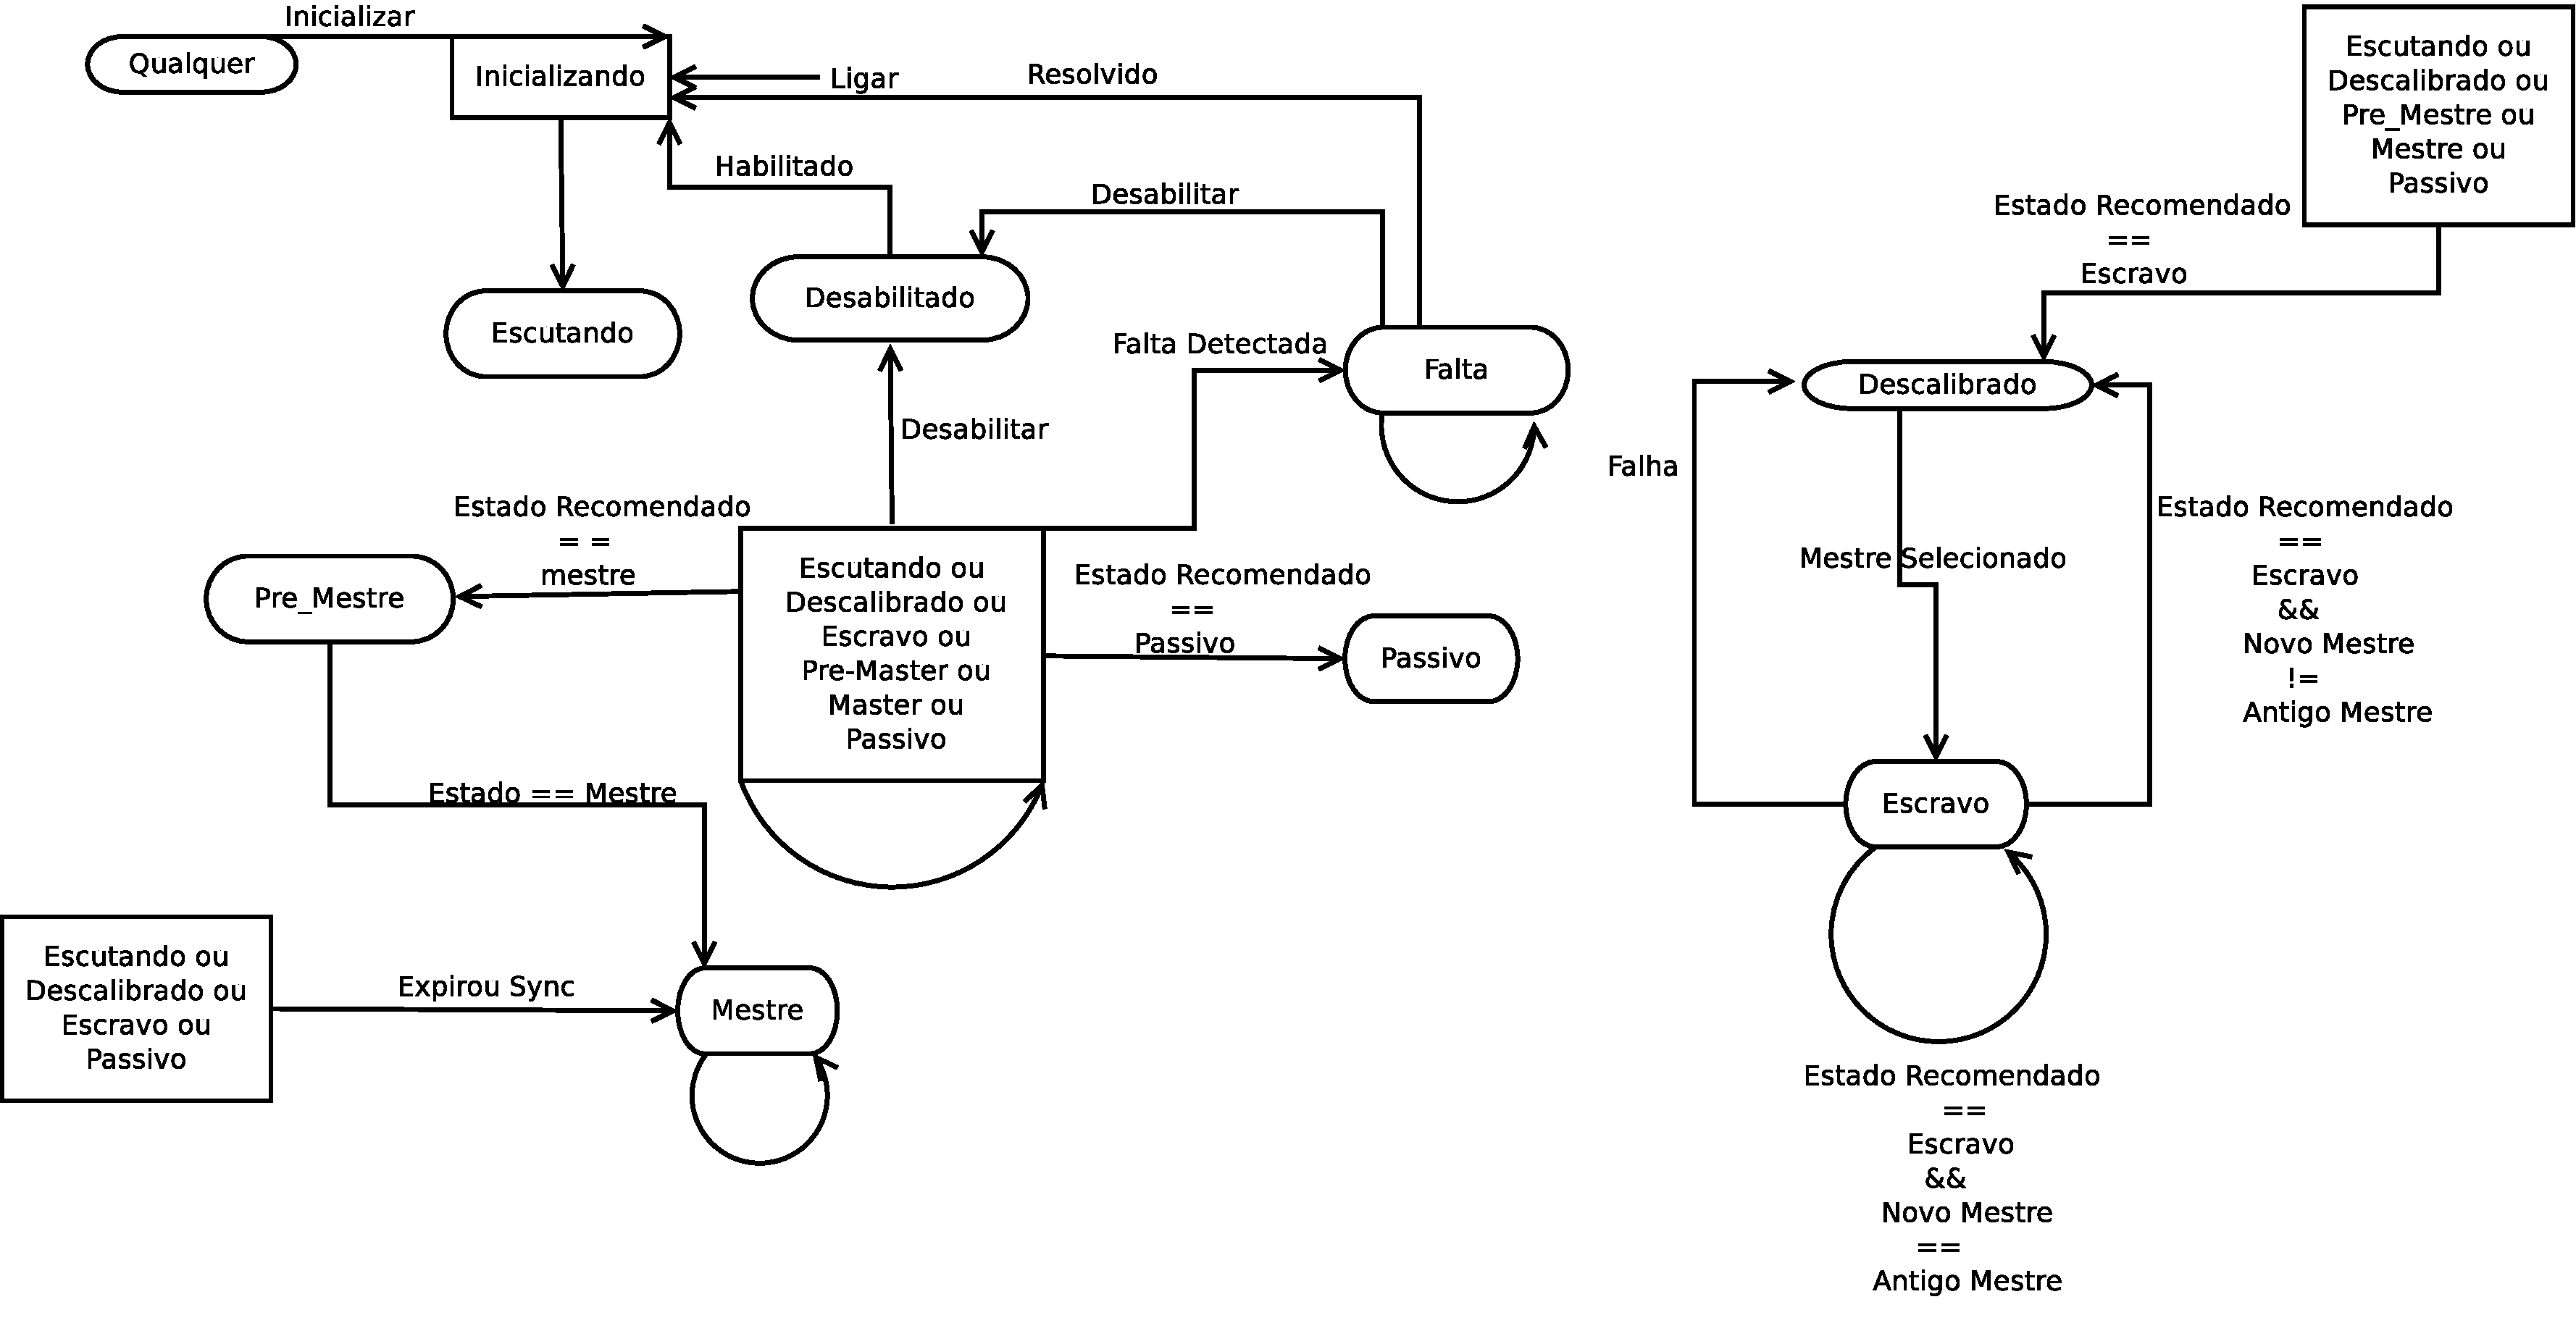
\includegraphics[scale=0.6, width=18cm]{fig/Maquina_de_Estados_do_Protocolo_IEEEE1588.pdf}
		\caption{Máquina de Estados do PTP}
		\end{center}
		\end{figure*}
